As various graph properties have been discussed and defined, we now apply these properties onto connected graphs to demonstrate their use. As well as this, they are used to outline and modify the graph such that an alternative layout may be given, revealing correlations between the vertices or edges within the graph. Through the use of Python, I have coded a program to display a graph either generated from a weighted matrix, a adjacency matrix or a graph data set that's pre-existing. To help accomplish this, I have used Tiago's Graph Tool library for python which contains useful documentation and functions to achieve the graph generations as well as other mathematical libraries for complex arithmetic. The general idea is to compare various graph properties by modifying their positions according to the values of their graph properties. For simplicity and the goal of being comparable, we choose the y-axis of the graph to be based upon the trophic coherence and the x-axis to vary between the different properties discussed in the last chapter.

\section{Early Experimentations}
By programming and using tools from the various libraries within python, I was able to generate graphs and define each property value based upon the generated graphs. Then the positioning of each vertex can be modified in relation to the values calculated.

Initially, out of the many pre-existing graphical datasets from Tiago's library, I experimented on a smaller dataset that demonstrates the relationships between karate clubs in a city so that I can test and generate a visualisation of this dataset. This dataset involved 34 karate clubs where the initial graph can be shown by Figure \ref{fig:karate} with the adjacency matrix in Appendix \ref{app:karateadj}.

\begin{figure}[H]
	\centering
	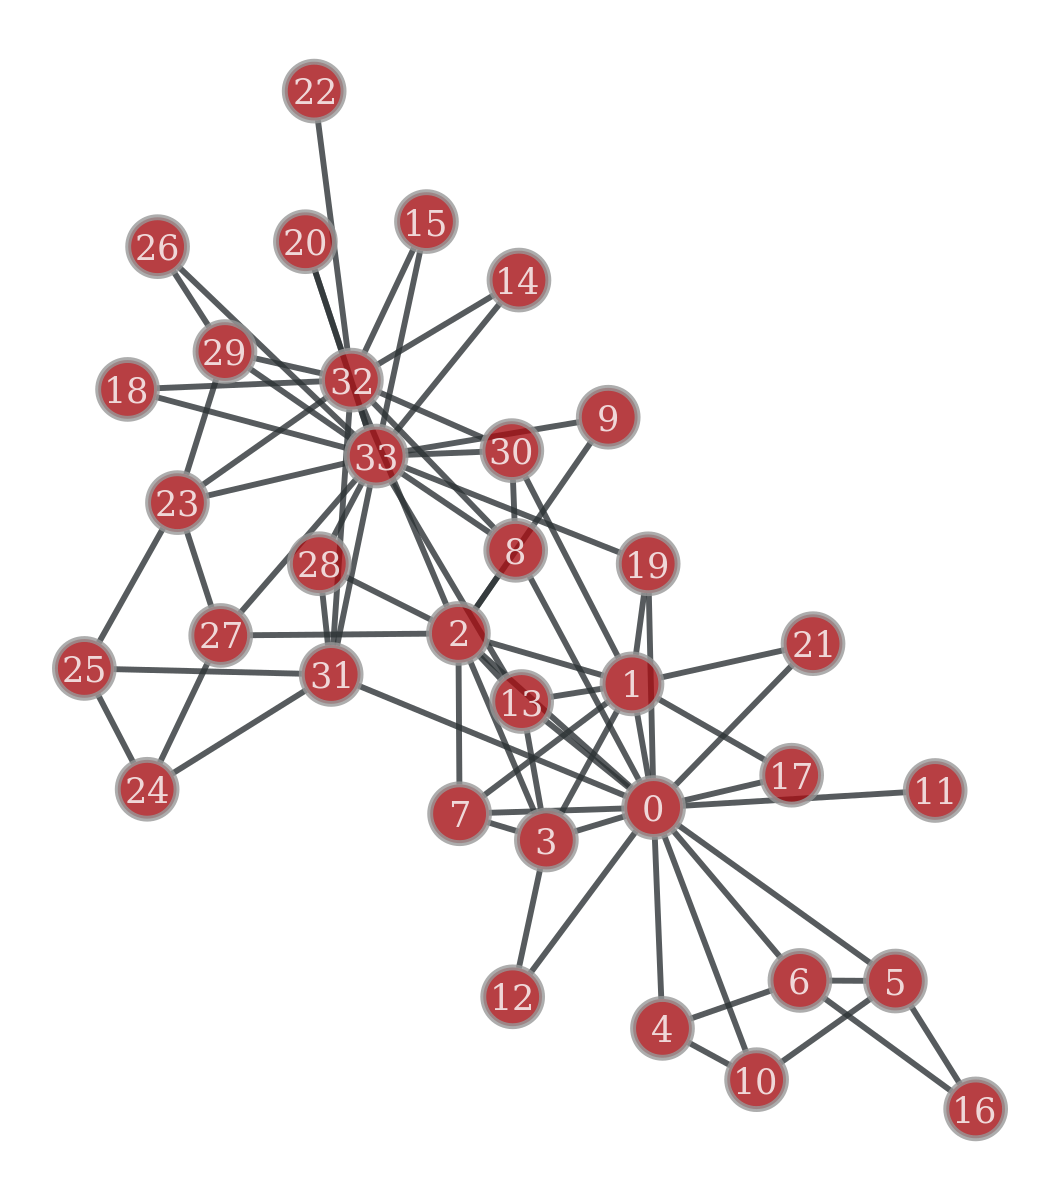
\includegraphics[scale=0.20]{karate.png}
	\caption{The initial graph based on the karate club dataset pre-existing within the library that was generated through the python program. Contains 34 clubs and their connections to one another with no important meaning with the positions of the vertices.}
	\label{fig:karate}
\end{figure}

Current positioning of the graph are determined based on the idea that the vertex do not overlap and the connections are all easily visible. So the dataset's positioning has no real benefits other than having good visibility. Any correlations or vital information can not be derived from the initial graph as the positions do not represent anything. The only information that can be derived easily are the certain outliers who only have one edge, vertices 22 and 11. The vertices that have more edges can also be seen such as vertices 32, 33 and 0 under closer examination. But these vertices are difficult to distinguish at a first glance. Thus, we now include various different graph properties discussed in the last chapter to ensure that more can be derived. This can be seen in Figures \ref{fig:karatecentrality} and \ref{fig:karatelocal} by using the trophic coherence values for each vertex as their y-value and another property value for their x-value.

For karate clubs, as the graph is not directed, the trophic levels do not represent a clear hierarchical format since there is no distinction between "upstream" or "downstream" of information with the edges of the graph. Consequently, the vertices in the karate graph do not have information that passes in one direction. So for vertices such as 1 or 16, they could be recognised as the start or end of the network hence the reason they have the largest and smallest trophic levels. Even if the flow of information is bidirectional, trophic levels are still useful in implementing some structure into the karate dataset. Further datasets involving languages that will be explored will be directional so that trophic levels can be used optimally.

\begin{figure}[H]
\centering
\begin{subfigure}{.45\textwidth}
	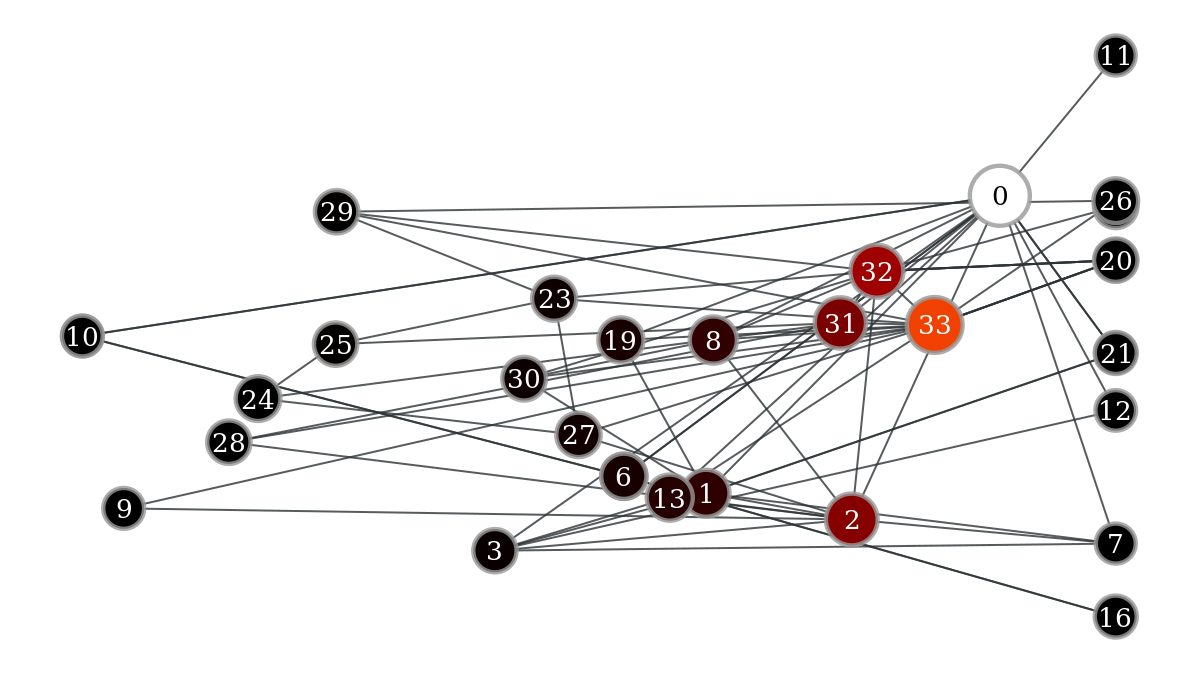
\includegraphics[scale=0.20]{karatebetween.png}
	\caption{Graph generated by karate dataset, the y-axis represents the trophic coherence values and the x-axis represents the betweenness centrality values for all the vertices. Additionally added colour changes between the x-axis to give a clearer visualisation of the separations.}
	\label{fig:karatea}
\end{subfigure}
\hfill
\begin{subfigure}{.45\textwidth}
	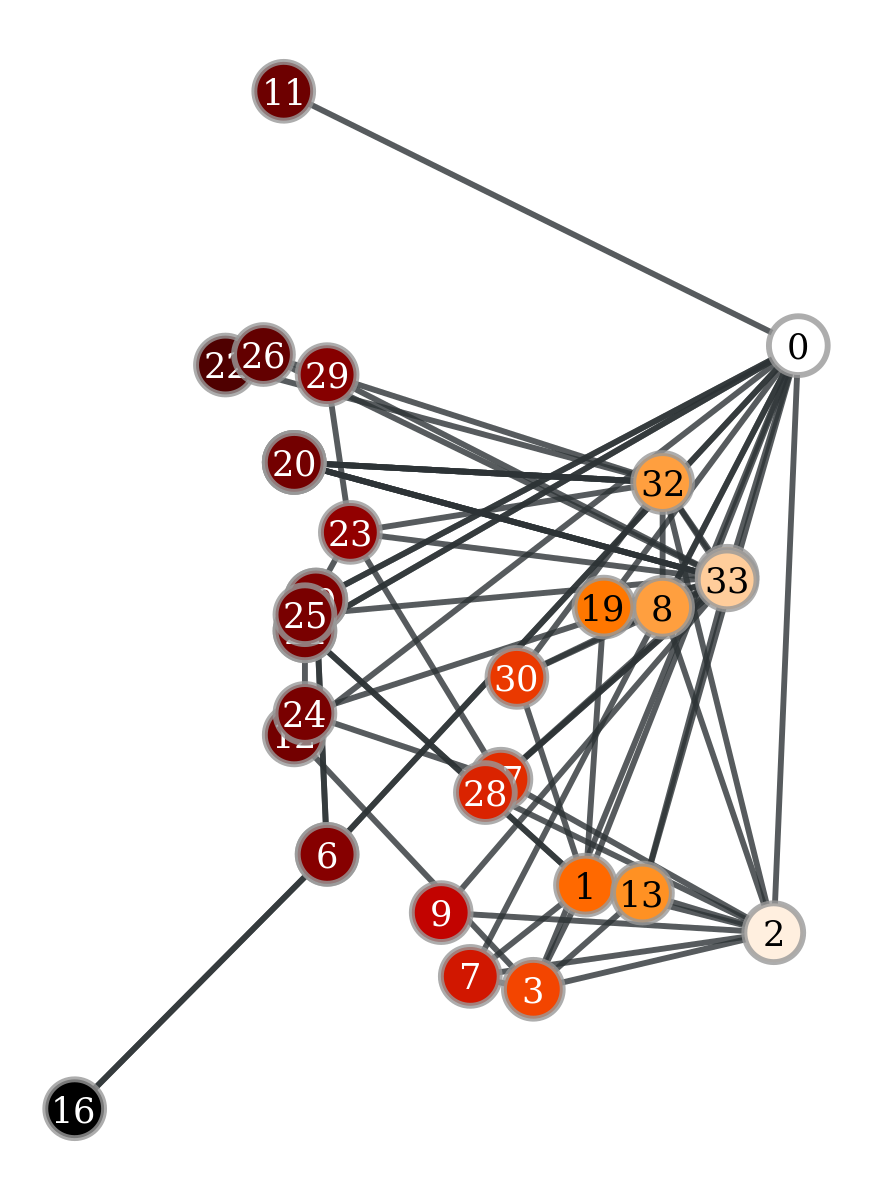
\includegraphics[scale=0.2]{karatecloseness.png}
	\caption{Graph generated similarly to the betweenness graph for the karate dataset but the vertices are plotted with local clustering coefficient as the x-axis and trophic levels as the y-axis.}
	\label{fig:karateb}
\end{subfigure}
\caption{Centrality values as the x-axis}
\label{fig:karatecentrality}
\end{figure}

Figure \ref{fig:karatea} shows the karate graph with the x-axis representing the betweenness value. The betweenness value are scaled by a factor or 10 to give a clearer visualisation with larger betweenness value further on the x-axis. Which also means the vertex is more frequently involved among short paths of the connections. In this case, the connections of the clubs. We can see that vertex 0 is the furthest right vertex so is involved in the most short paths between all the vertices of the karate graph. On the other hand, vertices such as 11, 7, 16 and more are clubs who are on the outskirts with no proper connections to other clubs. Can be seen on the left side on the figure. Therefore, in relation to this dataset, the clubs with larger betweenness are the clubs who are more centralised in a city and have more meaningful links to others.

We compare this to another centrality value, the closeness values who also has been scaled by a factor of 10. Figure \ref{fig:karateb} represents this in place of the betweenness value. Through comparison of both, vertices are positioned similarly to betweenness. This is because betweenness are values when considering all vertices within the graph whereas closeness considers all neighbours of a specific vertex. In other words, betweenness measured the control a vertex has over the flow of information through the entire graph, whereas closeness measures the control over the flow of information with vertices in close proximity (i.e. neighbours). Therefore the vertices on the right of both the betweenness and closeness graph would be the most important/largest clubs. Additionally, clubs such as 19 who have a larger closeness compared to betweenness means that it is important to the clubs in close proximity of itself, in other words, the club is the most important/largest within its local area.

\begin{figure}[H]
	\centering
	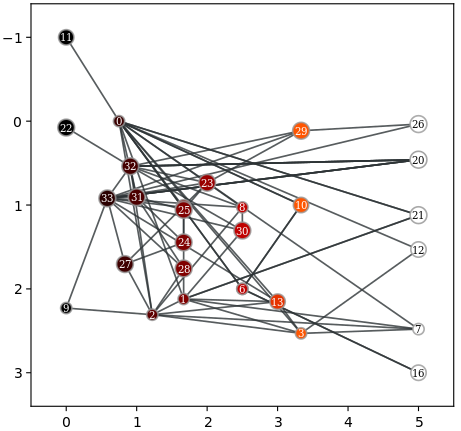
\includegraphics[scale=0.22]{karatelocal.png}
	\caption{Graph generated similarly to the betweenness graph for the karate dataset but the vertices are plotted with local clustering coefficient as the x-axis and trophic levels as the y-axis.}
	\label{fig:karatelocal}
\end{figure}


Figure \ref{fig:karatelocal} is shown with local clustering coefficient as the x-axis instead of betweenness. After manipulation the vertices positions, notice that the clubs with less connections to the major clubs (vertices of high degree) are visually seen to the left in both graphs as these vertices would have a low clustering coefficient as well as a low betweenness. On Figure \ref{fig:karatelocal}, the vertices with the best connections to major clubs are seen further to the right which we see are the karate clubs 26, 20 and 12 etc. However vertices with high betweenness seen before such as vertex 33 instead have a smaller local clustering as their club has connections to smaller clubs, decreasing the overall value of it's own connections. So this means that clubs on the right have quicker access/communication with better clubs and are the closest to them.

All the values for each club can be shown in table format, Table \ref{KarateTable}, where apart from the initial column, each column is one of the different graph property value.

\begin{table}[H]
    \centering
    \small
    \caption{Table containing all the values calculated for each vertex of the graph.. The order is in the club number depicted in the first column.}
    \begin{tabular}{|l|l|l|l|l|}
        \hline
        \textbf{Club} & \textbf{Trophic Levels} & \textbf{Betweenness} & \textbf{Closeness} & \textbf{Local Clustering} \\ \hline
        0 & 0 & 0.437645803 & 0.568965517 & 0.15 \\ \hline
        1 & 2.12094015 & 0.053873557 & 0.485294118 & 0.333333333 \\ \hline
        2 & 2.30804964 & 0.152263709 & 0.559322034 & 0.244444444 \\ \hline
        3 & 2.53039414 & 0.011961881 & 0.464788732 & 0.666666667 \\ \hline
        4 & 1 & 0.000631313 & 0.379310345 & 0.666666667 \\ \hline
        5 & 2 & 0.029987374 & 0.38372093 & 0.5 \\ \hline
        6 & 2 & 0.029987374 & 0.38372093 & 0.5 \\ \hline
        7 & 2.47969196 & 0 & 0.44 & 1 \\ \hline
        8 & 1.02851103 & 0.056737013 & 0.515625 & 0.5 \\ \hline
        9 & 2.22893206 & 0.000847763 & 0.428571429 & 0 \\ \hline
        10 & 1 & 0.000631313 & 0.379310345 & 0.666666667 \\ \hline
        11 & -1 & 0 & 0.366666667 & 0 \\ \hline
        12 & 1.53039414 & 0 & 0.370786517 & 1 \\ \hline
        13 & 2.15210654 & 0.04159151 & 0.507692308 & 0.6 \\ \hline
        14 & 0.45900156 & 0 & 0.370786517 & 1 \\ \hline
        15 & 0.45900156 & 0 & 0.370786517 & 1 \\ \hline
        16 & 3 & 0 & 0.284482759 & 1 \\ \hline
        17 & 1.12094015 & 0 & 0.375 & 1 \\ \hline
        18 & 0.45900156 & 0 & 0.370786517 & 1 \\ \hline
        19 & 1.02788172 & 0.02936057 & 0.492537313 & 0.333333333 \\ \hline
        20 & 0.45900156 & 0 & 0.370786517 & 1 \\ \hline
        21 & 1.12094015 & 0 & 0.375 & 1 \\ \hline
        22 & 0.07623827 & 0 & 0.34375 & 0 \\ \hline
        23 & 0.73415591 & 0.018244949 & 0.392857143 & 0.4 \\ \hline
        24 & 1.44596889 & 0.002209596 & 0.375 & 0.333333333 \\ \hline
        25 & 1.05781988 & 0.003840488 & 0.375 & 0.333333333 \\ \hline
        26 & 0.03492233 & 0 & 0.358695652 & 1 \\ \hline
        27 & 1.70452843 & 0.02170214 & 0.452054795 & 0.166666667 \\ \hline
        28 & 1.75702472 & 0.001794733 & 0.445945946 & 0.333333333 \\ \hline
        29 & 0.1140399 & 0.003869048 & 0.38372093 & 0.666666667 \\ \hline
        30 & 1.30422637 & 0.014727633 & 0.458333333 & 0.5 \\ \hline
        31 & 0.90660502 & 0.140348425 & 0.540983607 & 0.2 \\ \hline
        32 & 0.53811913 & 0.182157888 & 0.515625 & 0.181818182 \\ \hline
        33 & 0.92088243 & 0.275055616 & 0.540983607 & 0.116666667 \\ \hline
    \end{tabular}
    \label{KarateTable}
\end{table}

This is the early experimentations of the positioning of vertices within the graph so instead of using simple datasets, I will generate the datasets based upon various different languages as well as their sentence structure. To understand this further, words in languages must be given a rank which can be demonstrated through Zipf's Law discussed in the next section.

\section{Zipf's Law}
Zipf's law analyses the natural languages and the frequency of words that appear in them. Alternatively, Zipf's Law\cite{hosch2009zipf} is generally seen as the frequencys of specific events are inversely proportional to their rank that is determined through this law. The law was proposed by George Kinbgsley Zipf when researching the various frequencies of words within the English language. The law states that the $r^{\text{th}}$ most frequent word in the language has a frequency of $f(r)$ that has a relation with the inverse of $r$ where r is the \emph{frequency rank} for the word and $f(r)$ as the frquency of the word in the corpus examined (The \emph{corpus} means the collection of written text).

\begin{equation}\label{eq:zipfs}
f(r) \propto \frac{1}{r^{\alpha}}
\end{equation}

This is the scale for $\alpha \approx 1$ and means that the most frequent word in the examined text which is $r = 1$ has it's frequency of appearance to 1, the next most frequent word which is $r = 2$ has a frequency appearane of $\frac{1}{2^{\alpha}}$ and so on. This Zipf's law can be drawn on a graph to show a relation and when $log(f)$ is drawn against $log(r)$, the graph generates a curve that closely resembles a straight line with a slope of -1. This is known as Zipf's curve and later in the 1960s, this was reinforced by the law being correct for smaller corpora\cite{sicilia2002extension}. However the curve varies depending on the corpora as expected and the higher ranking words deviated more from the straight line. Therefore, Mandelbrot derived a generalisation for Zipf's law to adjust to the frequency distributions within the different languages. Mandelbrot proposed to adjust the rank by a constant $\beta$, demonstrated by

\begin{equation}\label{eq:zipfs}
f(r) \propto \frac{1}{(r + \beta)^{\alpha}}
\end{equation}

Generalisation of Zipf's law can then be applied to various different corpus of languages so that a frequency distribution can be viewed for the corpus. An example of this can be seen in Figure \ref{fig:zipfwiki}.

\begin{figure}[!htb]
	\centering
	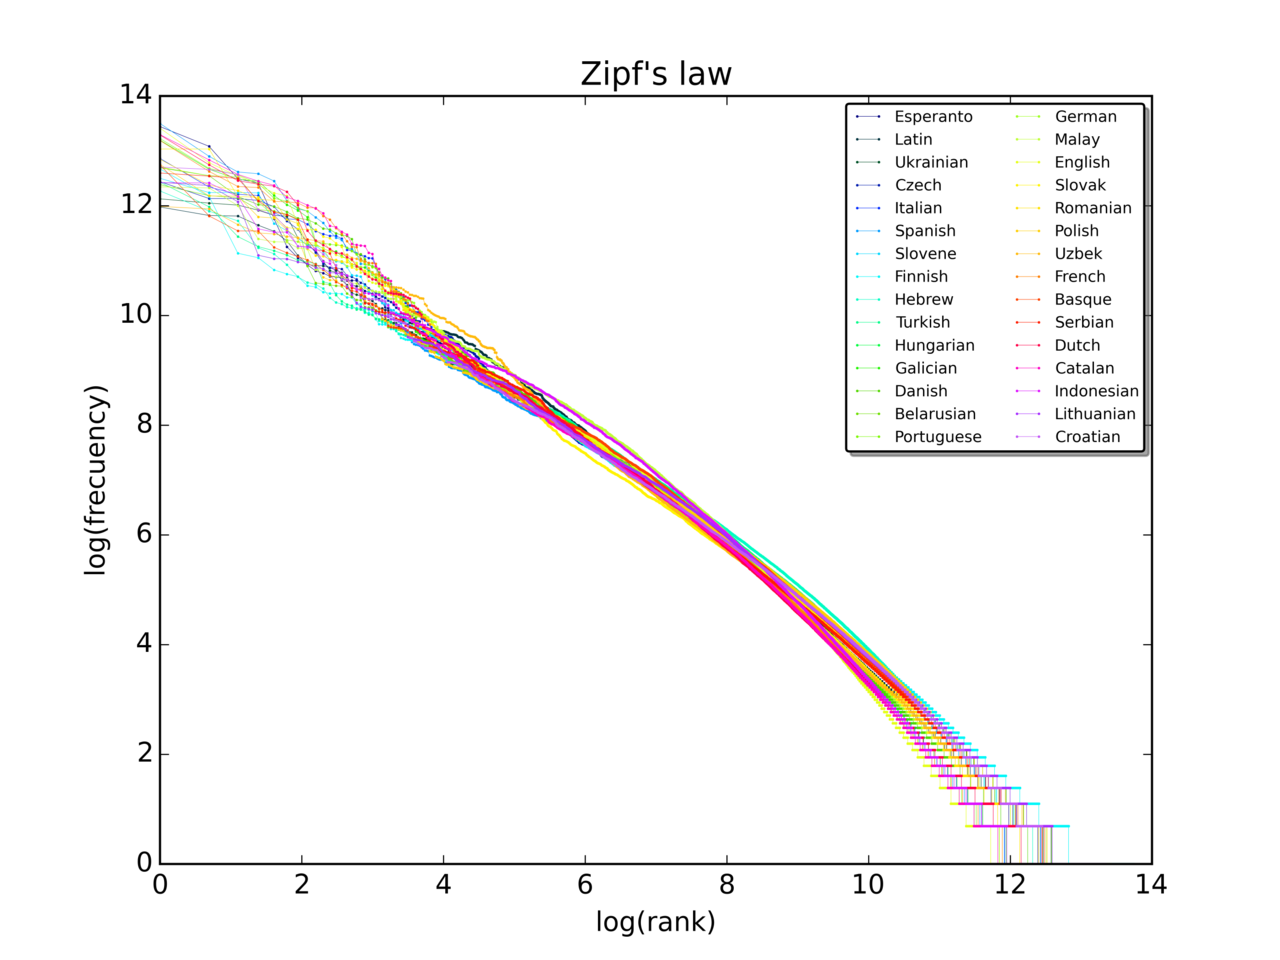
\includegraphics[scale=2.5]{zipfwiki.png}
	\caption{The plot of Zipf's law containing 30 different language corpus generated from the first 10 million words in each language from Wikipedias. The image was sourced from Wikipedia\cite{zipffigure}. }
	\label{fig:zipfwiki}
\end{figure}

So words in a corpus has a systematic relationship between their rank in their occurence table and their frequency that they appear in their corpus. Meaning that their are words within languages that are used more commonly such as "the", "or", "of" that account for most of the word occurences and other words such as "xylophone" and "accordion". A larger corpus is studied by Bentz, Kiela, Hill and Buttery \cite{BentzKielaHillButtery} where they study zipfs law for Old English and Modern English. They study the frequency and ranks of each word and then compare them between the old and new English. In doing so, for Old English, the words "and" is ranked first with a frequency of 1731 whereas in Modern English, "the" is ranked first with a frequency of 1775 and "and" is second instead with a frequency of 1024. By looking at more words and the comparisons between them, Old English has a larger number of distinct types whilst Modern English had less but this meant that they had higher frequencies within their first 100 words.
In conclusion Zipf's Law is a useful tool as languages tend to follow Zipf's curve in terms of their frequencies and rank meaning that by following an existing corpus of language, the data can be extrapolated and used in other corpus's to determine similarities between the known and the unknown texts. As well as to use it to determine the types of words that are deemed to be most common in a language. We will use Zipf's Law when comparing texts of different languages in further experiments. 


\begin{table}[]
\small
\begin{tabular}{|l|l|l|l|l|l|l|l|l|l|}
\hline
\textbf{a}             & 7 & 0        & 0.28174  & 0        & \textbf{kingdom}   & 1 & 0.027993 & 0.01017  & 0        \\ \hline
\textbf{acquaintances} & 1 & 0.135998 & 0.018304 & 0        & \textbf{left}      & 1 & 0.727384 & 0.009838 & 0        \\ \hline
\textbf{also}          & 1 & 0.303191 & 0.007227 & 0        & \textbf{lived}     & 1 & -0.19525 & 0.01559  & 0        \\ \hline
\textbf{and}           & 9 & 0.253523 & 0.304283 & 0.057143 & \textbf{lives}     & 1 & 0.618904 & 0.022175 & 0        \\ \hline
\textbf{as}            & 2 & 0.242183 & 0.022354 & 0.333333 & \textbf{might}     & 1 & 0.417113 & 0.008503 & 0        \\ \hline
\textbf{bathing}       & 1 & -0.18498 & 0.047444 & 0        & \textbf{none}      & 1 & 1.364857 & 0        & 0        \\ \hline
\textbf{be}            & 3 & 0.449879 & 0.095843 & 0        & \textbf{not}       & 2 & -0.49384 & 0.064906 & 0        \\ \hline
\textbf{beautiful}     & 1 & 0.326277 & 0.023314 & 0        & \textbf{of}        & 4 & 0.801328 & 0.188965 & 0        \\ \hline
\textbf{before}        & 1 & 0.14996  & 0.025352 & 0        & \textbf{on}        & 1 & 0.428216 & 0.012338 & 0        \\ \hline
\textbf{bid}           & 1 & 0.28077  & 0.011625 & 0        & \textbf{once}      & 1 & 0.26579  & 0.00544  & 0        \\ \hline
\textbf{bore}          & 1 & 0.113036 & 0.022239 & 0        & \textbf{one}       & 1 & 0.714174 & 0.0224   & 0        \\ \hline
\textbf{bring}         & 1 & 0        & 0.059647 & 0        & \textbf{only}      & 2 & -0.02083 & 0.062283 & 0        \\ \hline
\textbf{but}           & 3 & 0.018472 & 0.03931  & 0        & \textbf{ordained}  & 1 & 0.054413 & 0.016009 & 0        \\ \hline
\textbf{by}            & 1 & 0        & 0.058069 & 0        & \textbf{other}     & 1 & 0.592159 & 0.029245 & 0        \\ \hline
\textbf{came}          & 1 & -0.19525 & 0.01559  & 0        & \textbf{out}       & 2 & 1.004888 & 0.074518 & 0        \\ \hline
\textbf{child}         & 2 & 1.293955 & 0        & 0        & \textbf{past}      & 1 & -0.38382 & 0.021713 & 0        \\ \hline
\textbf{contain}       & 1 & -0.29869 & 0.034392 & 0        & \textbf{plates}    & 1 & 0.069116 & 0.032401 & 0        \\ \hline
\textbf{could}         & 1 & -0.16199 & 0.06438  & 0        & \textbf{provided}  & 1 & 0.001655 & 0.030823 & 0        \\ \hline
\textbf{daughter}      & 2 & -0.19599 & 0.043738 & 0        & \textbf{queen}     & 3 & 0.226072 & 0.093925 & 0.1      \\ \hline
\textbf{day}           & 1 & 0.731605 & 0.030297 & 0        & \textbf{relations} & 1 & 0.109517 & 0.019819 & 0        \\ \hline
\textbf{did}           & 1 & 0.043998 & 0.022204 & 0        & \textbf{said}      & 2 & 0.908794 & 0.050292 & 0        \\ \hline
\textbf{each}          & 1 & 0.522436 & 0.028719 & 0        & \textbf{shall}     & 1 & 0.450446 & 0.030297 & 0        \\ \hline
\textbf{eat}           & 1 & 0.539867 & 0.021348 & 0        & \textbf{shalt}     & 1 & 0        & 0.059121 & 0        \\ \hline
\textbf{every}         & 1 & 0.661882 & 0.029771 & 0        & \textbf{so}        & 2 & 0.216075 & 0.049709 & 0        \\ \hline
\textbf{favourable}    & 1 & 0.353118 & 0.035284 & 0        & \textbf{squatted}  & 1 & 0.268522 & 0.011812 & 0        \\ \hline
\textbf{feast}         & 1 & 2        & 0        & 0        & \textbf{that}      & 4 & 0.436479 & 0.106106 & 0.03714 \\ \hline
\textbf{for}           & 2 & 0.091603 & 0.078154 & 0        & \textbf{the}       & 9 & 0.587911 & 0.279782 & 0.044118 \\ \hline
\textbf{foretold}      & 1 & 0.351014 & 0.015958 & 0        & \textbf{their}     & 1 & 0.710116 & 0.021649 & 0        \\ \hline
\textbf{friends}       & 1 & 0.18152  & 0.020345 & 0        & \textbf{them}      & 3 & 0.228276 & 0.153123 & 0.1      \\ \hline
\textbf{frog}          & 2 & 0.485953 & 0.079587 & 0        & \textbf{there}     & 3 & -0.39051 & 0.079992 & 0        \\ \hline
\textbf{from}          & 1 & 0.627021 & 0.021874 & 0        & \textbf{they}      & 2 & 0.384346 & 0.045086 & 0        \\ \hline
\textbf{fulfilled}     & 1 & 0.29992  & 0.024826 & 0        & \textbf{thirteen}  & 1 & 0.404049 & 0.030297 & 0        \\ \hline
\textbf{golden}        & 1 & 0.046629 & 0.031875 & 0        & \textbf{thou}      & 1 & 0        & 0.058595 & 0        \\ \hline
\textbf{gone}          & 1 & 0        & 0.057543 & 0        & \textbf{thy}       & 1 & 0.45158  & 0.029245 & 0        \\ \hline
\textbf{great}         & 1 & 1        & 0.009888 & 0        & \textbf{times}     & 1 & -0.37713 & 0.021187 & 0        \\ \hline
\textbf{ground}        & 1 & 0.420717 & 0.018217 & 1        & \textbf{to}        & 6 & 0.452713 & 0.227705 & 0.018182 \\ \hline
\textbf{had}           & 4 & 0.364857 & 0.16175  & 0.035714 & \textbf{twelve}    & 1 & 0.024142 & 0.031349 & 0        \\ \hline
\textbf{happened}      & 2 & 0.095101 & 0.032509 & 0        & \textbf{was}       & 1 & 0.020545 & 0.046918 & 0        \\ \hline
\textbf{has}           & 1 & 0        & 0.057017 & 0        & \textbf{water}     & 1 & 0.420717 & 0.018217 & 1        \\ \hline
\textbf{he}            & 4 & 0.108827 & 0.112105 & 0.047619 & \textbf{we}        & 1 & 0.400668 & 0.019524 & 0        \\ \hline
\textbf{her}           & 1 & 0.452146 & 0.028719 & 0        & \textbf{were}      & 1 & 0.006771 & 0.029771 & 0        \\ \hline
\textbf{himself}       & 1 & -0.10354 & 0.034918 & 0        & \textbf{when}      & 1 & 0.512195 & 0        & 1        \\ \hline
\textbf{his}           & 2 & 0.037515 & 0.039246 & 0        & \textbf{who}       & 1 & 0.567433 & 0.005729 & 0        \\ \hline
\textbf{in}            & 2 & -0.37045 & 0.039218 & 0        & \textbf{wise}      & 1 & 0.537434 & 0.02267  & 0        \\ \hline
\textbf{into}          & 1 & 0.195961 & 0.011039 & 0        & \textbf{wish}      & 1 & 0.451013 & 0.029771 & 0        \\ \hline
\textbf{it}            & 3 & 0.382995 & 0.062455 & 0        & \textbf{women}     & 1 & 0.486956 & 0.023196 & 0        \\ \hline
\textbf{joy}           & 1 & 0.172563 & 0.023776 & 0        & \textbf{world}     & 1 & 1.587911 & 0        & 0        \\ \hline
\textbf{kind}          & 1 & 0.351701 & 0.042138 & 0        & \textbf{would}     & 1 & 0.527692 & 0.022701 & 0        \\ \hline
\textbf{king}          & 2 & 0.169862 & 0.176086 & 0.166667 & \textbf{year}      & 1 & 0        & 0.056491 & 0        \\ \hline
\end{tabular}
\end{table}
\begin{table}[!ht]
    \centering
    \setlength\tabcolsep{2pt}
    \begin{tabular}{lllllllllllllll}
        0 & 1 & 1 & 1 & 1 & 1 & 1 & 1 & 1 & 0 & 1 & 1 & 1 & 1 & 0 \\ 
        1 & 0 & 1 & 1 & 0 & 0 & 0 & 1 & 0 & 0 & 0 & 0 & 0 & 1 & 0 \\ 
        1 & 1 & 0 & 1 & 0 & 0 & 0 & 1 & 1 & 1 & 0 & 0 & 0 & 1 & 0 \\ 
        1 & 1 & 1 & 0 & 0 & 0 & 0 & 1 & 0 & 0 & 0 & 0 & 1 & 1 & 0 \\ 
        1 & 0 & 0 & 0 & 0 & 0 & 1 & 0 & 0 & 0 & 1 & 0 & 0 & 0 & 0 \\ 
        1 & 0 & 0 & 0 & 0 & 0 & 1 & 0 & 0 & 0 & 1 & 0 & 0 & 0 & 0 \\ 
        1 & 0 & 0 & 0 & 1 & 1 & 0 & 0 & 0 & 0 & 0 & 0 & 0 & 0 & 0 \\ 
        1 & 1 & 1 & 1 & 0 & 0 & 0 & 0 & 0 & 0 & 0 & 0 & 0 & 0 & 0 \\ 
        1 & 0 & 1 & 0 & 0 & 0 & 0 & 0 & 0 & 0 & 0 & 0 & 0 & 0 & 0 \\ 
        0 & 0 & 1 & 0 & 0 & 0 & 0 & 0 & 0 & 0 & 0 & 0 & 0 & 0 & 0 \\ 
        1 & 0 & 0 & 0 & 1 & 1 & 0 & 0 & 0 & 0 & 0 & 0 & 0 & 0 & 0 \\ 
        1 & 0 & 0 & 0 & 0 & 0 & 0 & 0 & 0 & 0 & 0 & 0 & 0 & 0 & 0 \\ 
        1 & 0 & 0 & 1 & 0 & 0 & 0 & 0 & 0 & 0 & 0 & 0 & 0 & 0 & 0 \\ 
        1 & 1 & 1 & 1 & 0 & 0 & 0 & 0 & 0 & 0 & 0 & 0 & 0 & 0 & 0 \\ 
        0 & 0 & 0 & 0 & 0 & 0 & 0 & 0 & 0 & 0 & 0 & 0 & 0 & 0 & 0 \\ 
        0 & 0 & 0 & 0 & 0 & 0 & 0 & 0 & 0 & 0 & 0 & 0 & 0 & 0 & 0 \\ 
        0 & 0 & 0 & 0 & 0 & 1 & 1 & 0 & 0 & 0 & 0 & 0 & 0 & 0 & 0 \\ 
        1 & 1 & 0 & 0 & 0 & 0 & 0 & 0 & 0 & 0 & 0 & 0 & 0 & 0 & 0 \\ 
        0 & 0 & 0 & 0 & 0 & 0 & 0 & 0 & 0 & 0 & 0 & 0 & 0 & 0 & 0 \\ 
        1 & 1 & 0 & 0 & 0 & 0 & 0 & 0 & 0 & 0 & 0 & 0 & 0 & 0 & 0 \\ 
        0 & 0 & 0 & 0 & 0 & 0 & 0 & 0 & 0 & 0 & 0 & 0 & 0 & 0 & 0 \\ 
        1 & 1 & 0 & 0 & 0 & 0 & 0 & 0 & 0 & 0 & 0 & 0 & 0 & 0 & 0 \\ 
        0 & 0 & 0 & 0 & 0 & 0 & 0 & 0 & 0 & 0 & 0 & 0 & 0 & 0 & 0 \\ 
        0 & 0 & 0 & 0 & 0 & 0 & 0 & 0 & 0 & 0 & 0 & 0 & 0 & 0 & 0 \\ 
        0 & 0 & 0 & 0 & 0 & 0 & 0 & 0 & 0 & 0 & 0 & 0 & 0 & 0 & 0 \\ 
        0 & 0 & 0 & 0 & 0 & 0 & 0 & 0 & 0 & 0 & 0 & 0 & 0 & 0 & 0 \\ 
        0 & 0 & 0 & 0 & 0 & 0 & 0 & 0 & 0 & 0 & 0 & 0 & 0 & 0 & 0 \\ 
        0 & 0 & 1 & 0 & 0 & 0 & 0 & 0 & 0 & 0 & 0 & 0 & 0 & 0 & 0 \\ 
        0 & 0 & 1 & 0 & 0 & 0 & 0 & 0 & 0 & 0 & 0 & 0 & 0 & 0 & 0 \\ 
        0 & 0 & 0 & 0 & 0 & 0 & 0 & 0 & 0 & 0 & 0 & 0 & 0 & 0 & 0 \\ 
        0 & 1 & 0 & 0 & 0 & 0 & 0 & 0 & 1 & 0 & 0 & 0 & 0 & 0 & 0 \\ 
        1 & 0 & 0 & 0 & 0 & 0 & 0 & 0 & 0 & 0 & 0 & 0 & 0 & 0 & 0 \\ 
        0 & 0 & 1 & 0 & 0 & 0 & 0 & 0 & 1 & 0 & 0 & 0 & 0 & 0 & 1 \\ 
        0 & 0 & 0 & 0 & 0 & 0 & 0 & 0 & 1 & 1 & 0 & 0 & 0 & 1 & 1 \\ 
    \end{tabular}
\end{table}

\begin{table}[!ht]
    \centering
    \setlength\tabcolsep{2pt}
    \begin{tabular}{lllllllllllllllllll}
        0 & 0 & 1 & 0 & 1 & 0 & 1 & 0 & 0 & 0 & 0 & 0 & 0 & 0 & 0 & 0 & 1 & 0 & 0 \\ 
        0 & 0 & 1 & 0 & 1 & 0 & 1 & 0 & 0 & 0 & 0 & 0 & 0 & 0 & 0 & 1 & 0 & 0 & 0 \\ 
        0 & 0 & 0 & 0 & 0 & 0 & 0 & 0 & 0 & 0 & 0 & 0 & 1 & 1 & 0 & 0 & 0 & 1 & 0 \\ 
        0 & 0 & 0 & 0 & 0 & 0 & 0 & 0 & 0 & 0 & 0 & 0 & 0 & 0 & 0 & 0 & 0 & 0 & 0 \\ 
        0 & 0 & 0 & 0 & 0 & 0 & 0 & 0 & 0 & 0 & 0 & 0 & 0 & 0 & 0 & 0 & 0 & 0 & 0 \\ 
        0 & 1 & 0 & 0 & 0 & 0 & 0 & 0 & 0 & 0 & 0 & 0 & 0 & 0 & 0 & 0 & 0 & 0 & 0 \\ 
        0 & 1 & 0 & 0 & 0 & 0 & 0 & 0 & 0 & 0 & 0 & 0 & 0 & 0 & 0 & 0 & 0 & 0 & 0 \\ 
        0 & 0 & 0 & 0 & 0 & 0 & 0 & 0 & 0 & 0 & 0 & 0 & 0 & 0 & 0 & 0 & 0 & 0 & 0 \\ 
        0 & 0 & 0 & 0 & 0 & 0 & 0 & 0 & 0 & 0 & 0 & 0 & 0 & 0 & 0 & 1 & 0 & 1 & 1 \\ 
        0 & 0 & 0 & 0 & 0 & 0 & 0 & 0 & 0 & 0 & 0 & 0 & 0 & 0 & 0 & 0 & 0 & 0 & 1 \\ 
        0 & 0 & 0 & 0 & 0 & 0 & 0 & 0 & 0 & 0 & 0 & 0 & 0 & 0 & 0 & 0 & 0 & 0 & 0 \\ 
        0 & 0 & 0 & 0 & 0 & 0 & 0 & 0 & 0 & 0 & 0 & 0 & 0 & 0 & 0 & 0 & 0 & 0 & 0 \\ 
        0 & 0 & 0 & 0 & 0 & 0 & 0 & 0 & 0 & 0 & 0 & 0 & 0 & 0 & 0 & 0 & 0 & 0 & 0 \\ 
        0 & 0 & 0 & 0 & 0 & 0 & 0 & 0 & 0 & 0 & 0 & 0 & 0 & 0 & 0 & 0 & 0 & 0 & 1 \\ 
        0 & 0 & 0 & 0 & 0 & 0 & 0 & 0 & 0 & 0 & 0 & 0 & 0 & 0 & 0 & 0 & 0 & 1 & 1 \\ 
        0 & 0 & 0 & 0 & 0 & 0 & 0 & 0 & 0 & 0 & 0 & 0 & 0 & 0 & 0 & 0 & 0 & 1 & 1 \\ 
        0 & 0 & 0 & 0 & 0 & 0 & 0 & 0 & 0 & 0 & 0 & 0 & 0 & 0 & 0 & 0 & 0 & 0 & 0 \\ 
        0 & 0 & 0 & 0 & 0 & 0 & 0 & 0 & 0 & 0 & 0 & 0 & 0 & 0 & 0 & 0 & 0 & 0 & 0 \\ 
        0 & 0 & 0 & 0 & 0 & 0 & 0 & 0 & 0 & 0 & 0 & 0 & 0 & 0 & 0 & 0 & 0 & 1 & 1 \\ 
        0 & 0 & 0 & 0 & 0 & 0 & 0 & 0 & 0 & 0 & 0 & 0 & 0 & 0 & 0 & 0 & 0 & 0 & 1 \\ 
        0 & 0 & 0 & 0 & 0 & 0 & 0 & 0 & 0 & 0 & 0 & 0 & 0 & 0 & 0 & 0 & 0 & 1 & 1 \\ 
        0 & 0 & 0 & 0 & 0 & 0 & 0 & 0 & 0 & 0 & 0 & 0 & 0 & 0 & 0 & 0 & 0 & 0 & 0 \\ 
        0 & 0 & 0 & 0 & 0 & 0 & 0 & 0 & 0 & 0 & 0 & 0 & 0 & 0 & 0 & 0 & 0 & 1 & 0 \\ 
        0 & 0 & 0 & 0 & 0 & 0 & 0 & 0 & 0 & 0 & 1 & 0 & 1 & 0 & 1 & 0 & 0 & 1 & 1 \\ 
        0 & 0 & 0 & 0 & 0 & 0 & 0 & 0 & 0 & 0 & 1 & 0 & 1 & 0 & 0 & 0 & 1 & 0 & 0 \\ 
        0 & 0 & 0 & 0 & 0 & 0 & 0 & 0 & 1 & 1 & 0 & 0 & 0 & 0 & 0 & 0 & 1 & 0 & 0 \\ 
        0 & 0 & 0 & 0 & 0 & 0 & 0 & 0 & 0 & 0 & 0 & 0 & 0 & 0 & 1 & 0 & 0 & 0 & 1 \\ 
        0 & 0 & 0 & 0 & 0 & 0 & 0 & 0 & 1 & 1 & 0 & 0 & 0 & 0 & 0 & 0 & 0 & 0 & 1 \\ 
        0 & 0 & 0 & 0 & 0 & 0 & 0 & 0 & 0 & 0 & 0 & 0 & 0 & 0 & 0 & 0 & 1 & 0 & 1 \\ 
        0 & 0 & 0 & 0 & 0 & 0 & 0 & 0 & 1 & 0 & 0 & 1 & 0 & 0 & 0 & 0 & 0 & 1 & 1 \\ 
        0 & 0 & 0 & 0 & 0 & 0 & 0 & 0 & 0 & 0 & 0 & 0 & 0 & 0 & 0 & 0 & 0 & 1 & 1 \\ 
        0 & 0 & 0 & 0 & 0 & 0 & 0 & 0 & 0 & 1 & 1 & 0 & 0 & 1 & 0 & 0 & 0 & 1 & 1 \\ 
        1 & 0 & 0 & 1 & 0 & 1 & 0 & 1 & 1 & 0 & 0 & 0 & 0 & 0 & 1 & 1 & 1 & 0 & 1 \\ 
        1 & 0 & 0 & 1 & 1 & 1 & 0 & 0 & 1 & 0 & 0 & 1 & 1 & 1 & 1 & 1 & 1 & 1 & 0 \\ 
    \end{tabular}
\end{table}
\newpage
\newpage
\newpage
$\begin{pmatrix}
0 \\ 
0 \\
0 \\
0 \\
0 \\
0 \\
0 \\
0 \\
0 \\
0 \\
0 \\
0 \\
0 \\
0 \\
0 \\
0 \\
0 \\
0 \\
0 \\
0 \\
0 \\
0 \\
0 \\
0 \\
0 \\
0 \\
0 \\
0 \\
0 \\
0 \\
0 \\
0 \\
0 \\
0 \\
\end{pmatrix}$